% Условная компиляция для самостоятельной работы
\ifdefined\mainfile
    % Если это часть основного файла, не добавляем начало и конец документа
\else
    \documentclass[12pt, a4paper]{report}
    \usepackage{/Users/vladbelousov/Desktop/Semestr_4-FP-NSU/Настройка/library}
    \usepackage[utf8]{inputenc} % Подключение поддержки UTF-8
    \begin{document}
\fi

%%-------------------------------%%

\[ I = 2 \frac{I_0 }{a_s } \left( a_s + \frac{\sin \left( \frac{\omega_0 d }{c } \left[ \frac{x_s}{L_s} + \frac{x}{L }   \right]  \right)  \bigg | ^{\frac{a_s}{2 } }_{-\frac{a_s}{2 } } }{\frac{\omega_0 d }{c L_s} }  \right) = 2 I_0 \left( 1  + \cos \left[ \frac{\omega_0}{c } \frac{xd}{L}  \right] \frac{\sin \left[ \frac{\omega_0 d }{c } \frac{a_s }{2 L_s }   \right]}{\frac{\omega_0 d a_s  }{2c L_s} }  \right)  =\] 
\[ = 2 I_0 \bigg( 1 + \cos  \underbrace{\left[ \frac{\omega_0}{c} \frac{x d }{L }   \right]}_{k \Delta r } \underbrace{ \mathrm{sinc } \text{ } \left[ \frac{\omega_0}{c }  \frac{d a_s}{2 L_s}  \right]}_{\text{верно, если } \Delta r \ll l_{\parallel}  } \bigg) \] 

\[ V = \frac{2I_0 (1+ |\mathrm{sinc}|)- 2I_0 (1 - |\mathrm{sinc}  |)}{2 I_0 (1 + |\mathrm{sinc}  |) + 2 I_0 (1 - |\mathrm{sinc}  |)} = \left\lvert \mathrm{sinc }  \left( \frac{\omega_0}{c} \frac{d a_s }{2 L_s}  \right)  \right\rvert   \] 
- вычислена в центре  интерференционной картине.

\begin{center}
    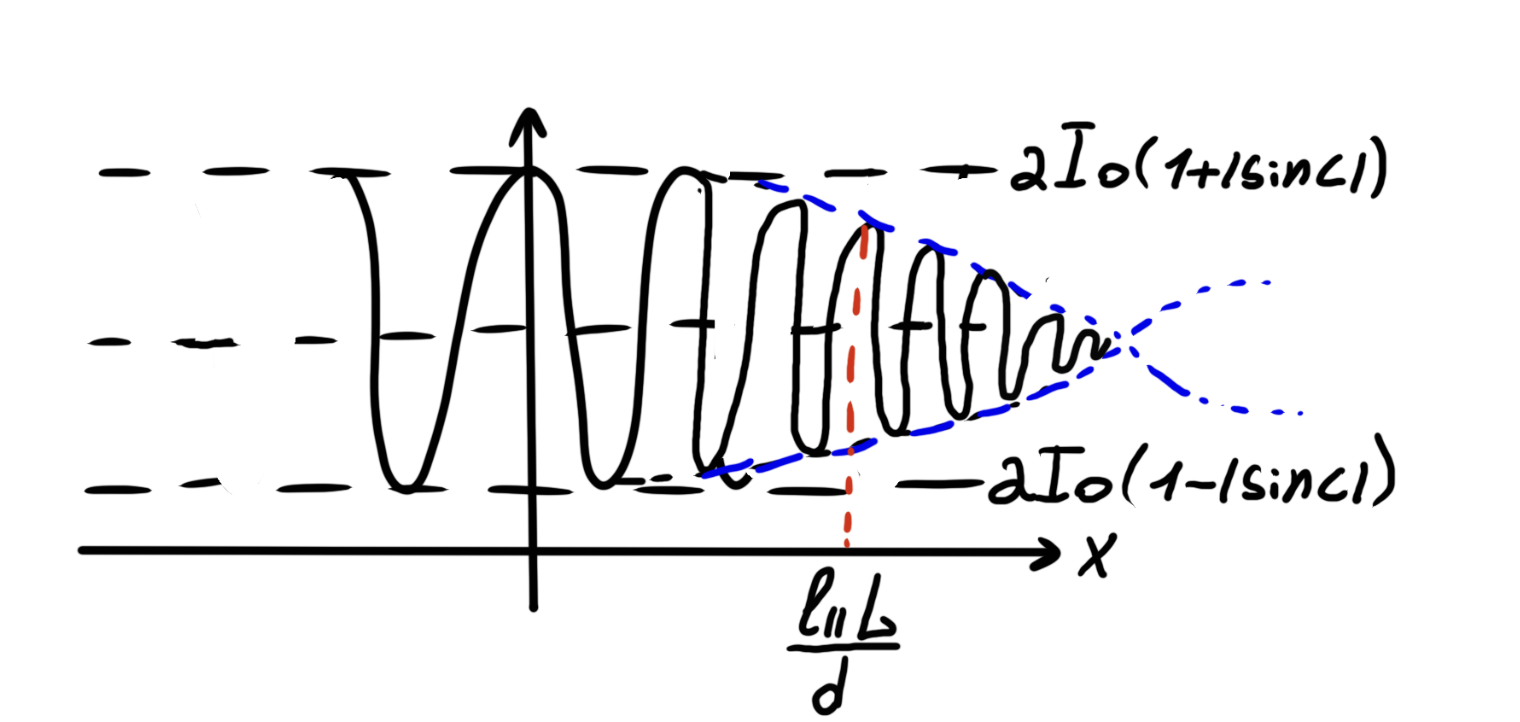
\includegraphics[width=0.6\textwidth]{/Users/vladbelousov/Desktop/Semestr_4-FP-NSU/ЭиО/Лекции_по_дням/image/124.png}
\end{center}  
Видность с ростом \( \Delta r  \) падает от 1 до 0.

\begin{center}
    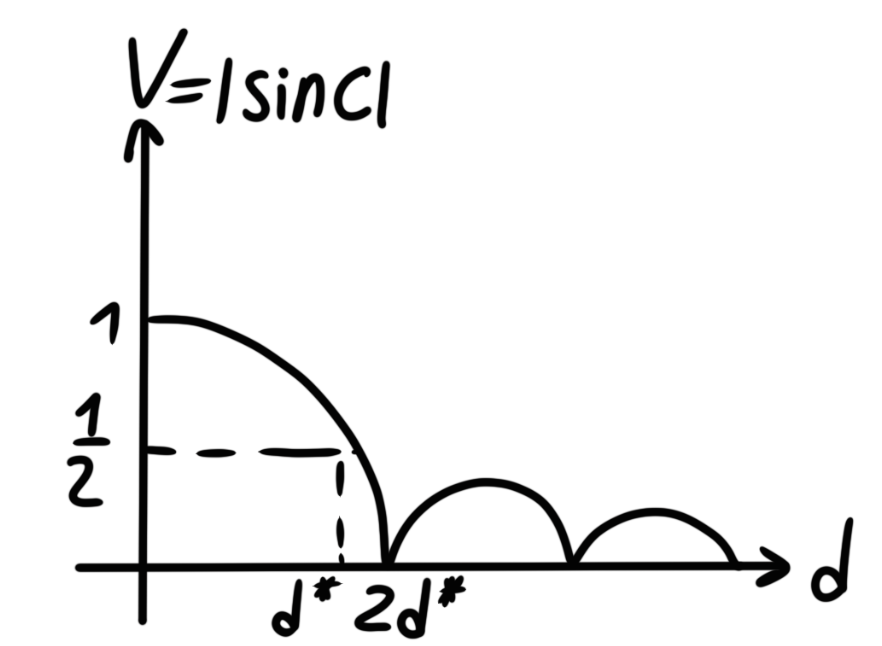
\includegraphics[width=0.4\textwidth]{/Users/vladbelousov/Desktop/Semestr_4-FP-NSU/ЭиО/Лекции_по_дням/image/118.png}
\end{center}  

\[ \frac{\omega_0}{c }  \frac{d^* a_s }{2 L_s } = \frac{\pi}{2 }  \Rightarrow d^* = \frac{\pi \lambda }{2 \pi \frac{a_s}{L_s}  } = \frac{\lambda}{2 \frac{a_s}{L_s}  }  = \frac{\lambda}{2 \theta}   \]
, где \( \theta  \) - угол под которым виден источник излучения из отверстия в экране, а \( d^* = l_{\perp } \) - поперечная длина когерентности   протяженного источника.

\[ \Delta r_s^* = \frac{d^* a_s }{2 L_s} = \frac{\lambda}{4}   \] 

Вывод: 

1) Немонохроматичность источника приводит к пространственному ограничению области, в которой наблюдается интерференционная картина \( (\Delta r < l_{\parallel} ) \);

2) Протяженность источника приводит к "размыванию" интерференционных полос, снижая их видность.

\section{Корреляционная функция случайного стационарного волнового поля}

\begin{center}
    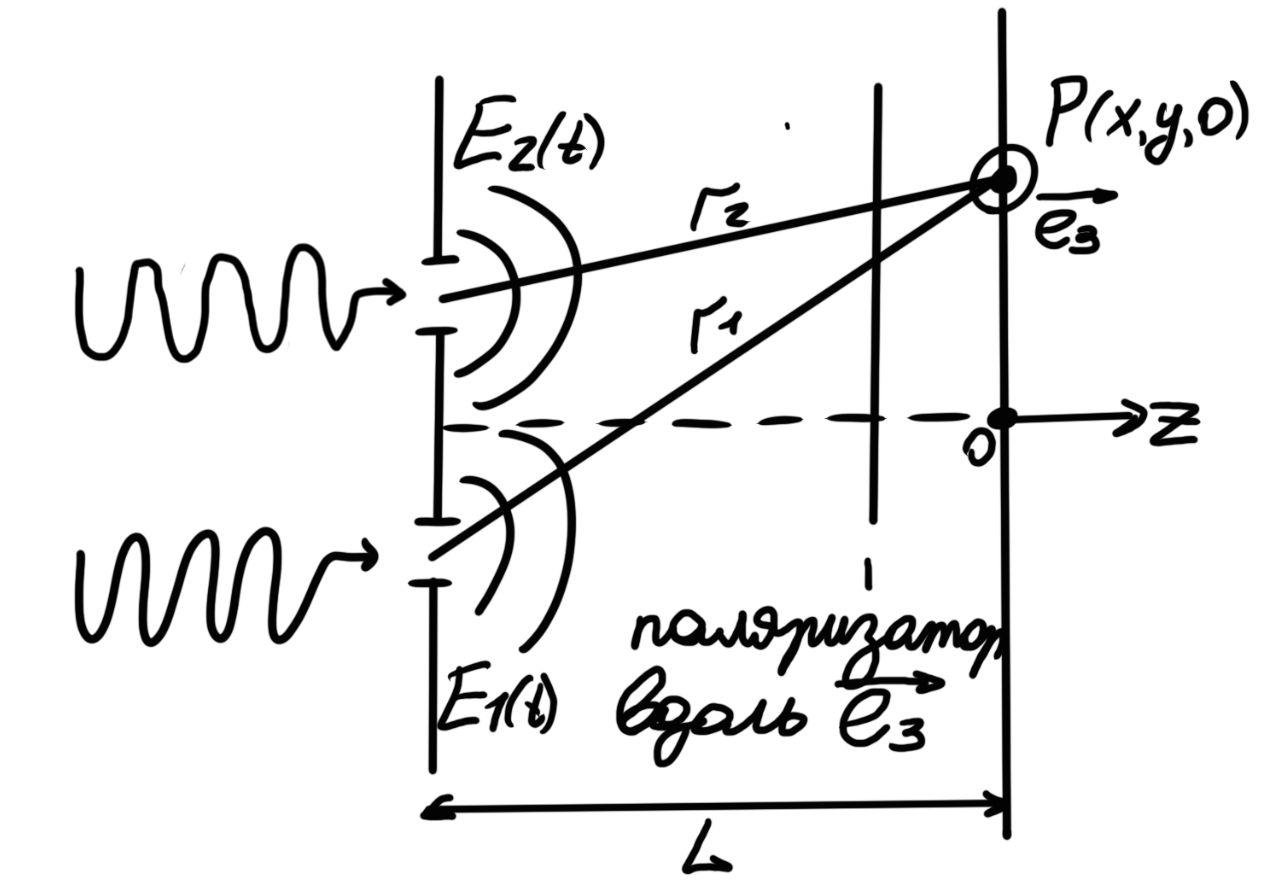
\includegraphics[width=0.5\textwidth]{/Users/vladbelousov/Desktop/Semestr_4-FP-NSU/ЭиО/Лекции_по_дням/image/119.png}
\end{center}  
\[ \vec{E } _1 (t ) \text{ и } \vec{E } _2 ( t ) \text{ - вещественные поля}  \] 

\[ \vec{E }  _{\Sigma}   = \vec{e }_3 \left(  \frac{\alpha}{r_1  } E_{1}\left( t - \frac{r_1}{c}  \right) + \frac{\alpha}{r_2 } E_2 \left( t - \frac{r_2}{c }  \right)    \right)  \text{ в точке } P  \] 

\[ I = <(\vec{E }  _{\Sigma } , \vec{E }  _{\Sigma }  )> = \frac{\alpha ^2 }{L ^2 } \bigg[ \underbrace{<E_1  ^2 \left( t - \frac{r_1}{c }  \right)>}_{I_1} + \underbrace{<E_2 ^2 \left( t - \frac{r_2}{c }  \right)>}_{I_2} + \underbrace{2 <E_1 \left( t - \frac{r_1}{c }     \right) E_2 \left( t - \frac{r_2}{c }  \right)>}_{I_{12}}\bigg]  \] 

\[ <E_1 \underbrace{\left( t - \frac{r_1}{c }  \right)}_{t ' } E_2 \left( t - \frac{r_2}{c }  \right)> = <E_1 (t )E_2 \bigg( t ' + \underbrace{\frac{\Delta r }{c}}_{\Delta t}  \bigg)> = <E_1 (t ') E_2 (t '+ \Delta t )> = G_{12 } ^{(0) }  (\Delta t)\]
, где \( G_{12 } ^{(0)}  \)  - корреляционная функция \( \displaystyle  \left( \Delta t = \frac{\Delta r }{c}  \right) \).

\[ I = \frac{\alpha  ^2  }{L ^2 } (G_{11 } ^{(0) } (0 ) + G_{22} ^{(0) }(0) + 2 G_{12} ^{(0 )}  (\Delta t ) )  = \frac{\alpha ^2 }{L ^2 } (G_{11}^{(0 )} +G_{22}^{(0 )}  + 2 \sqrt{G_{11}^{(0 )} G_{22}^{(0 )} } \gamma_{12} ^{(0)} (\Delta t ))  \] 
, где \( \gamma_{12} (\Delta t ) \)  - степень когерентности полей. 

\[ \gamma_{12} ^{(0 )}  = \frac{<E_1 (t ) E_2 (t + \Delta t )>}{\sqrt{<E_1 ^2 (t )><E_2 ^2 (t)>}}  \] 

Рассмотрим  квазимонохроматические поля \( E_1 (t ) = u_1 (t ) e^{ -  i \omega t    } , \text{ }  E_2(t ) = u_2 (t ) e^{- i \omega t }   \), где \( u_1 (t)\text{ и } u_2 (t) \in \mathbb{C}  \)  медленно меняются от времени.

\[<\mathrm{Re }  E_1 (t ) \mathrm{Re }  E_2(t + \Delta t )  >  = \bigg< \frac{ u_1 (t ) e^{ - i \omega t }+ u_1 ^* (t ) e^{i \omega t }  }{2} \cdot\frac{u_2 (t +\Delta t ) e^{ - i \omega (t + \Delta t ) }+ u_1 ^* (t + \Delta t ) e^{i \omega ( t + \Delta t )}  }{2} \bigg > =\] 
\[ \frac{ <u_1 (t ) u_2 ^{ * }  (t + \Delta t  ) >   e^{ i \omega \Delta t } +  u_1 ^{* }  u_2 (t + \Delta t  ) e^{ - i \omega \Delta t }  }{4}= \frac{1}{2 }  \mathrm{Re }  <u_1 (t ) u_2 ^* (t+ \Delta t ) >  e^{ i \omega \Delta t } \] 

\begin{center}
    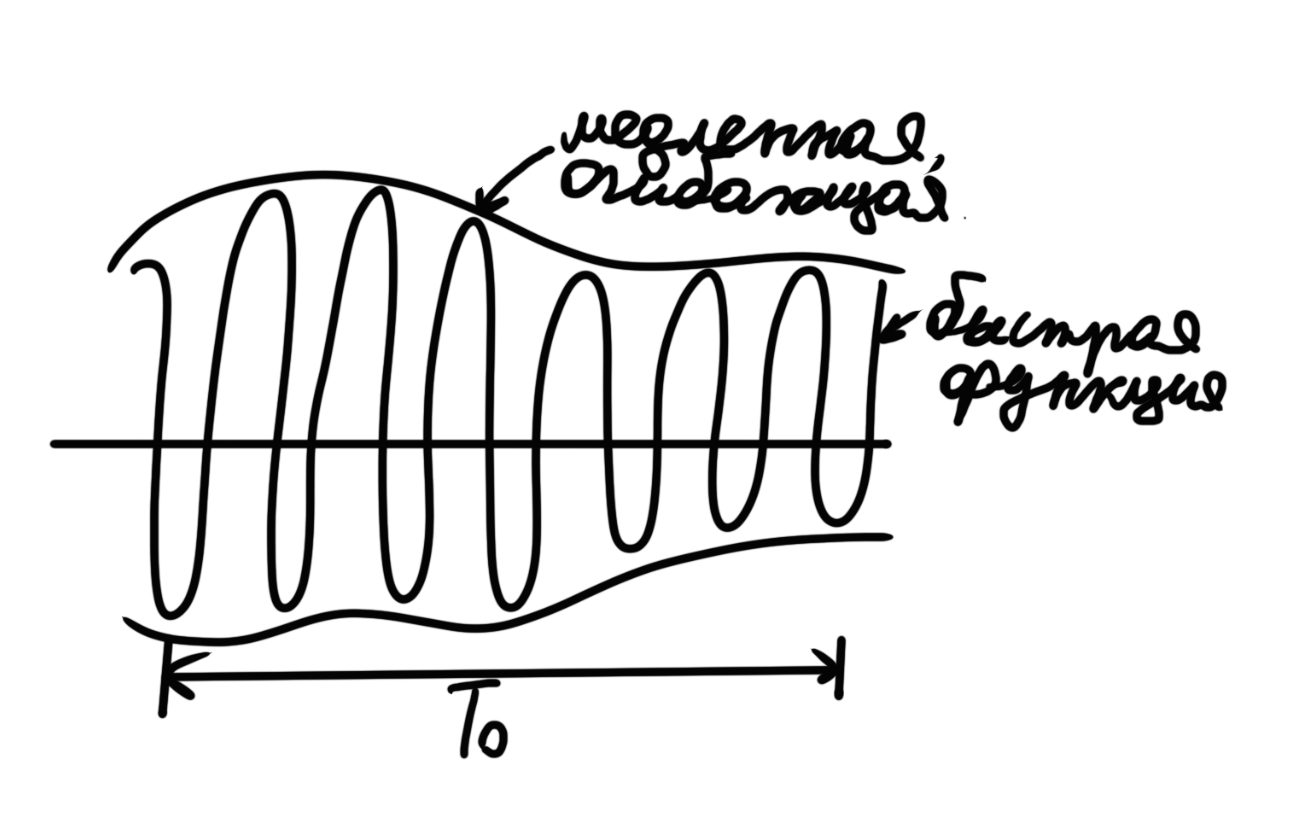
\includegraphics[width=0.5\textwidth]{/Users/vladbelousov/Desktop/Semestr_4-FP-NSU/ЭиО/Лекции_по_дням/image/120.png}
\end{center}  

\[ G_{12} (\Delta t ) = <u_1 (t ) u_2 ^* (t + \Delta t )> \text{ - корреляционная функция амплитуд полей.} \] 

\[ I = \frac{\alpha ^2 }{ 2 L ^2 } \bigg[  <|u_1 (t )| ^2 >+ <|u_2 (t)| ^2 >+ 2 \mathrm{Re }  {<u_1 (t ) u_2 ^* (t + \Delta t )>e ^{ i \omega \Delta t } }  \bigg]  = \] 
\[ = \frac{\alpha ^2 }{2 L ^2 } \bigg[ G_{11} ( 0 ) + G_{22} (0 ) + 2 \sqrt{G_{11} (0 ) G_{22} (0 )} \cdot \mathrm{Re }  \bigg( \frac{G_{12 } (\Delta t ) e^{ i \omega \Delta t }}{\underbrace{\sqrt{G_{11}(0 ) G_{22}(0 )}}_{\gamma_{12} ^{(0 )}  ( \Delta t )}}   \bigg)  \bigg]  \] 

\[ \gamma_{12} ^{(0 )}  (\Delta t ) = \frac{ |G_{12} (\Delta t ) | \cos ( \omega \Delta t + \arg  G_{12} (\Delta t ))}{ \sqrt{G_{11} (0 ) G_{22}(0)}}  , \text{ }  \gamma_{12} (\Delta t ) = \frac{ G_{12} (\Delta t )}{\sqrt{G_{11}(0 ) G_{22}(0 ) }} \]
, где \( \gamma_{12} (0 ) \) - комплексная степень когерентности амплитуд полей. 

\[ \gamma_{12}^{(0)}(\Delta t ) = |\gamma_{12} (\Delta t )| \cos (\omega \Delta t + \arg (\gamma_{12} (\Delta t ))) \] 

Для точечного квазимонохроматического источника в схеме Юнга: 

\[ I(\Delta t ) = 2 I_0     \bigg(1+ \cos (\omega_0 \Delta t ) \mathrm{ sinc } \left( \frac{\Delta \omega }{2 } \Delta t   \right) \bigg ) , \quad  I_1 = I_2 , \text{ }  \frac{\Delta r }{c } = \Delta t   \] 
\[ I(\Delta t ) = \frac{\alpha ^2 }{L ^2 } G_{11}(0 ) \bigg[1 + Re \bigg\{|\gamma_{11}(\Delta t) |\cos (\omega \Delta t + \arg \{\gamma_{11} (\Delta t)\})\bigg\}\bigg]  \] 
\[ \Rightarrow \gamma_{11} (\Delta t ) = \mathrm{sinc }  \left( \frac{\Delta \omega }{2 } \Delta t   \right)  \] 

Случай протяженного источника: 

\begin{center}
    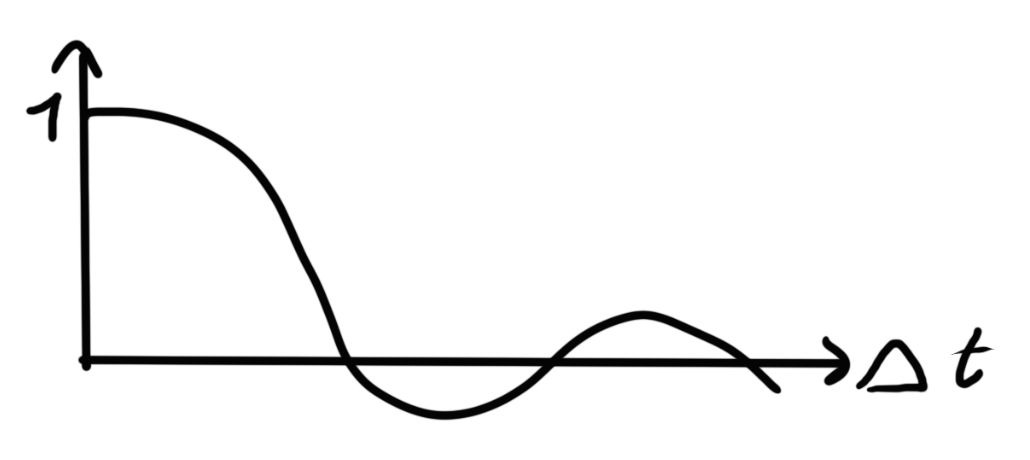
\includegraphics[width=0.5\textwidth]{/Users/vladbelousov/Desktop/Semestr_4-FP-NSU/ЭиО/Лекции_по_дням/image/121.png}
\end{center}  

\[ I( \Delta t )  = 2 I_0 \bigg(1 + \cos (\omega_0 \Delta t ) \mathrm{sinc }  \left( \frac{\omega_0 }{c } \frac{ d a_s }{2 L_s}   \right) \bigg) = 2 I_0 [1 + \cos (\omega_0 \Delta t + \arg (\mathrm{sinc }  )|\mathrm{sinc } (\text{ } ) |)] \] 
\[ \gamma_{11}(\Delta t \to  0 ) = \mathrm{sinc }  \left(  \frac{\omega_0 }{c } \frac{d a_s }{2 L_s}   \right)  \] 

Модель цугов со случайными фазами \( \varphi_0 ,\text{ }  \varphi_1 , \text{ }  \varphi_2 ,... \) 

\begin{center}
    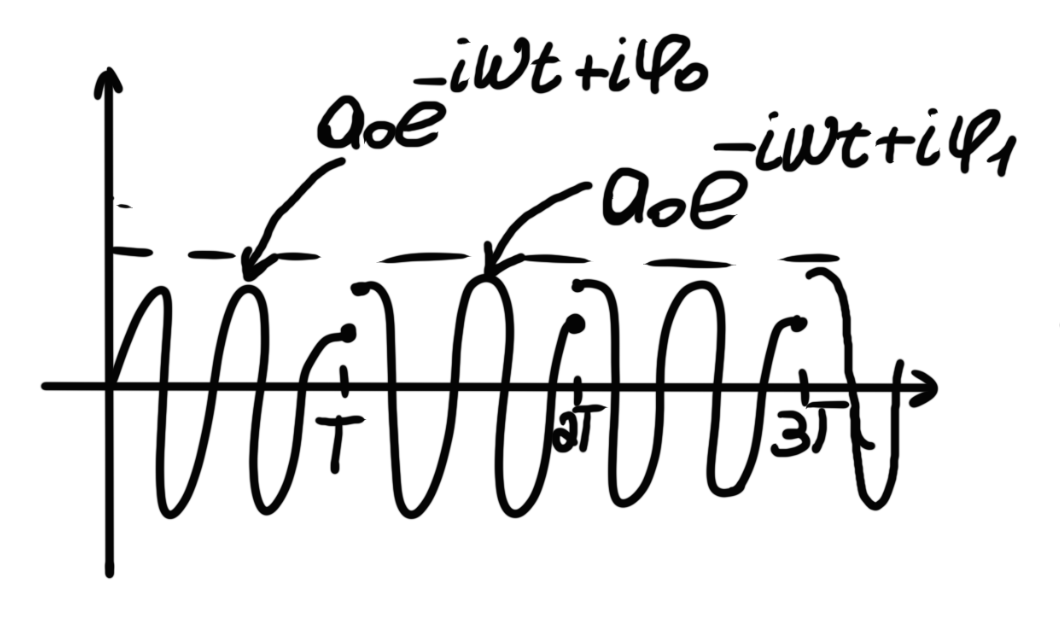
\includegraphics[width=0.4\textwidth]{/Users/vladbelousov/Desktop/Semestr_4-FP-NSU/ЭиО/Лекции_по_дням/image/122.png}
    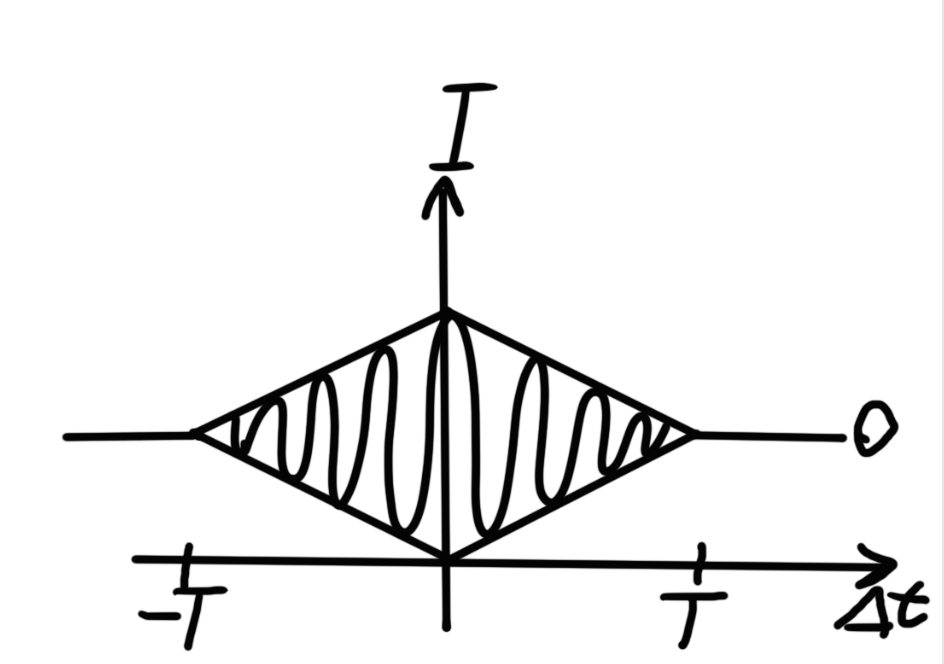
\includegraphics[width=0.4\textwidth]{/Users/vladbelousov/Desktop/Semestr_4-FP-NSU/ЭиО/Лекции_по_дням/image/123.png}
\end{center}  


%%-------------------------------%%

% Закрытие документа, если файл компилируется отдельно
\ifdefined\mainfile
    % Если это основной файл, не нужно заканчивать документ
\else
    \end{document}
\fi

